\chapter{就业结构的转型}
\label{chapter:struct}
《创新发展战略》指出,国家通过大力支持创新型企业,加速科技进步和产业升级,不仅优化并提升了企业结构,也显著改变了各行业对人才的需求。随着创新型企业的崛起,对跨学科、复合型人才,尤其是具备技术开发与创新能力的高端人才的需求日益增加。在这一趋势下,企业的创业和变革成为推动就业结构调整的重要力量,不仅催生了大量与科技创新紧密相关的新兴职业,也推动劳动者技能的转型,为社会迈向更加智能化、高效化奠定了坚实基础。

\section{劳动生产率与失业人数现状}
近年来,中国的劳动生产率与失业率的波动呈现出较为复杂的变化趋势。基于CEIC的《中国劳动生产率》数据集和世界银行集团的《总失业人数(占劳动力总数的比例)(模拟劳工组织估计)》数据集,绘制出2013年至2024年间中国劳动生产率的年度变化情况(见图\ref{中国劳动生产率}),以及中国、美国、日本、英国、法国等主要国家自1990年以来的失业率对比情况(见图\ref{主要国家失业率对比})。
\begin{figure}[H]
    \centering
    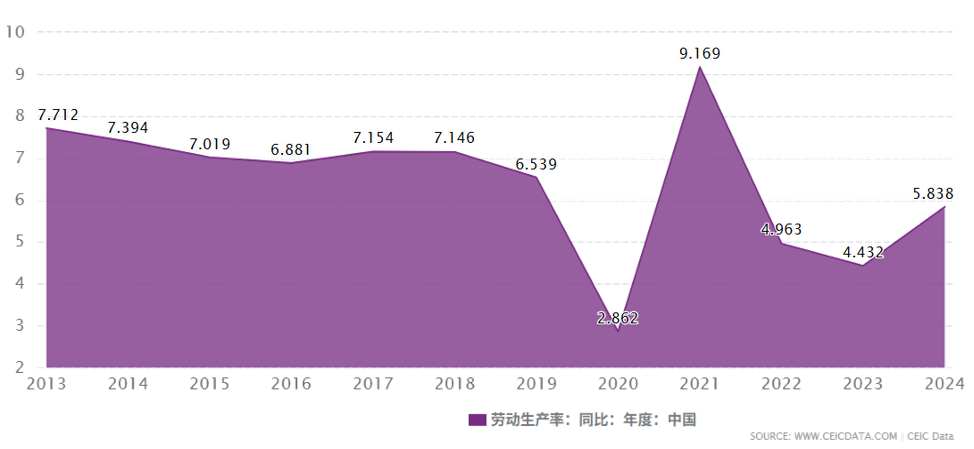
\includegraphics[width=0.7\linewidth]{figure/15中国劳动生产率.png}
    \caption{中国劳动生产率面积图}
    \label{中国劳动生产率}
\end{figure}
通过对图\ref{中国劳动生产率}的观察,可以清晰地看到中国劳动生产率这些年来波动明显,尤以2020年和2021年期间的剧烈波动为代表。数据充分表明,劳动生产率的波动受外部经济环境和国内政策的共同影响:2020年疫情对经济活动构成了巨大冲击,而2021年全球经济的复苏则带来了短期内的反弹。总体而言,尽管短期内波动较大,但在全球经济复苏及国内政策推动下,未来中国劳动生产率有望逐步进入稳定增长轨道。
\begin{figure}[H]
    \centering
    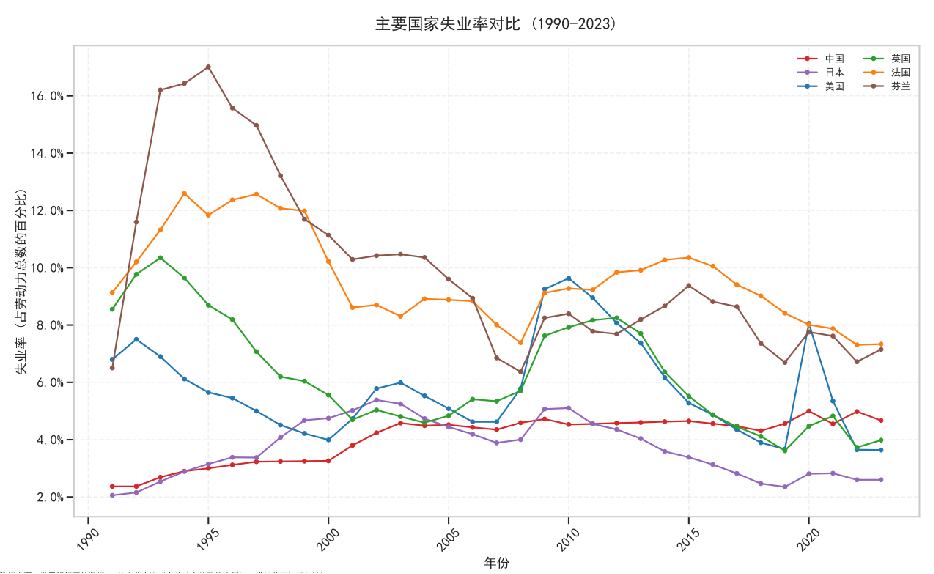
\includegraphics[width=0.7\linewidth]{figure/16主要国家失业率对比.png}
    \caption{主要国家失业率对比图}
    \label{主要国家失业率对比}
\end{figure}
同时,从图\ref{主要国家失业率对比}中可以看出,各国在不同时间段内的失业率变化各具特色。尤其是在1990年代中期和2008年全球金融危机期间,多国失业率均出现明显波动,这些波动反映了全球经济动荡对各国就业市场的深远影响。与此相比,中国的失业率总体呈现平稳上升的趋势,即使在2020年全球疫情爆发时曾短暂上升,但在政府有效政策调控下,很快得以控制,保持在较低水平,显示出较强的经济韧性与调适能力。

总体来看,劳动生产率的提升一直是中国经济转型的重要标志。与此同时,随着产业升级和自动化、智能化技术的不断推进,低技能岗位正逐步被新技术替代,导致部分领域的失业压力加大,尤其体现在年轻人和低技能工人群体中。如何在推动高技术岗位发展的同时,有效应对传统岗位的减少,是当前亟需解决的挑战。\cite{zhang2022digital}

\section{科技创新促进就业结构转型}
随着科技创新特别是人工智能、大数据、云计算等技术的普及,全球劳动市场、就业市场的结构发生了深刻变化。特别是在中国,科技创新推动了许多新兴行业的发展,尤其是在第三产业(服务业)中。传统制造业和农业中低技能岗位的减少,使得高技能岗位的需求逐步增加。

\subsection{全球人工智能岗位趋势}
AI岗位作为技术密集型职位,随着全球对人工智能技术的需求不断上升,已成为各国劳动市场中极为重要的一部分。基于和鲸平台数据集,制作出“2014-2023年各个地区人工智能(AI)相关岗位所占总岗位比例的变化情况”折线图(见图\ref{各个地区人工智能(AI)相关岗位所占总岗位比例的变换情况图})。

\begin{figure}[H]
    \centering
    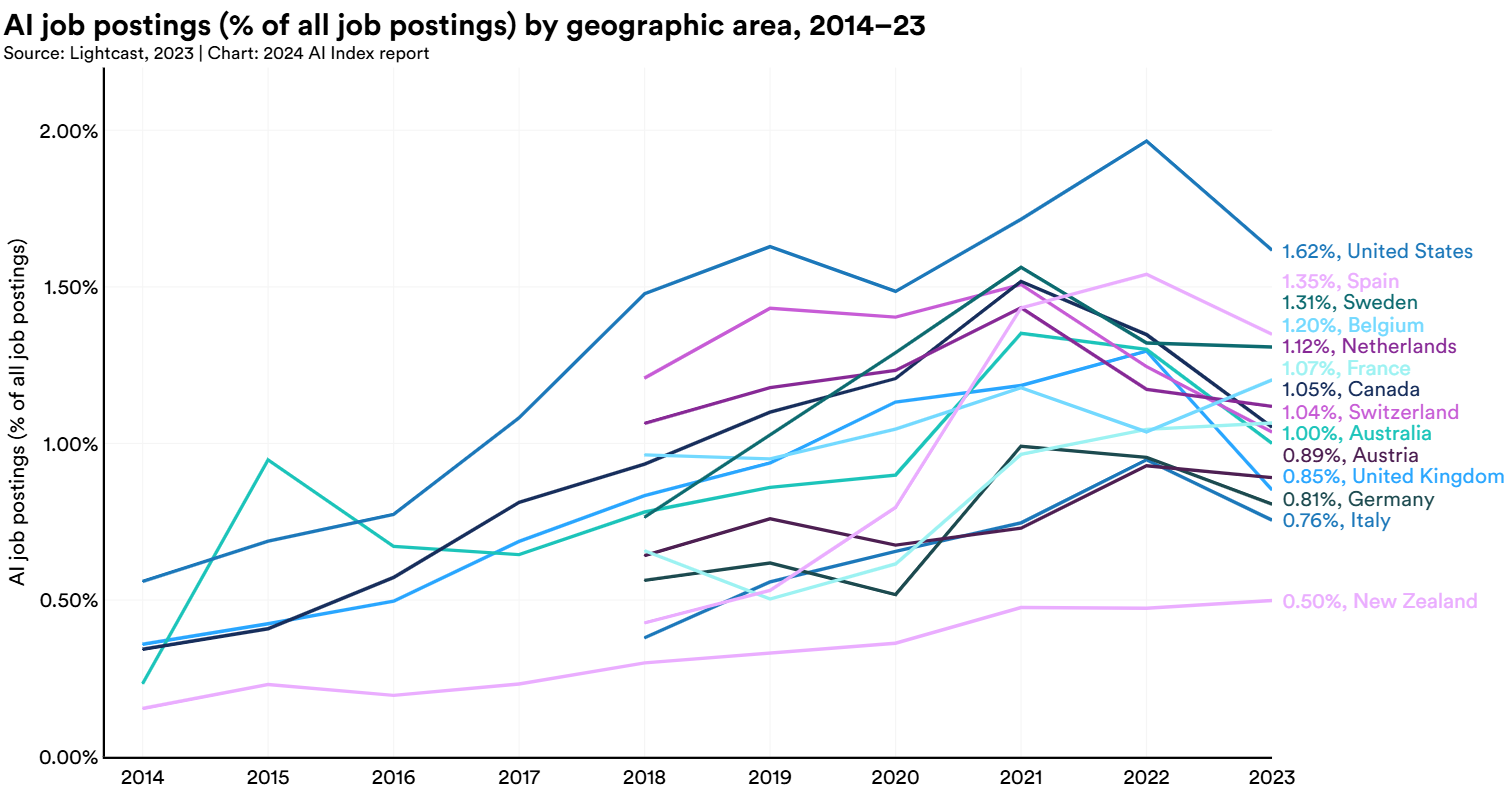
\includegraphics[width=0.7\linewidth]{figure/17各个地区人工智能(AI)相关岗位所占总岗位比例的变换情况图.png}
    \caption{各个地区人工智能(AI)相关岗位所占总岗位比例的变换情况图}
    \label{各个地区人工智能(AI)相关岗位所占总岗位比例的变换情况图}
\end{figure}

该图清晰地展示了2014年至2023年期间,各国AI岗位占比的逐年变化。全球人工智能岗位比例总体呈上升趋势,但在2023年出现了下降,这表明市场对人工智能技术的投资与需求可能正经历阶段性调整,行业不断成熟和竞争加剧使得岗位增长趋于理性。

展望未来,随着技术创新不断深入,人工智能岗位将成为全球劳动力市场的重要组成部分,尤其在高技术行业中的应用将进一步拓展。各国需要加大对AI技术研发的投入,并加强人才培养,以迎接即将到来的技术变革。\cite{wang2024impact}

\subsection{全球AI岗位发布情况}
在当前快速发展的科技环境中,人工智能(AI)正逐步改变全球劳动力市场的格局。随着AI技术的广泛应用,各组织对于AI对员工数量和工作结构的影响产生了不同的预期。根据和鲸平台数据集,展示出2023年,基于麦肯锡和公司调查数据,未来3年人工智能对组织劳动力影响的预期(见图\ref{未来3年人工智能对组织劳动力影响的预期图})。
\begin{figure}[H]
    \centering
    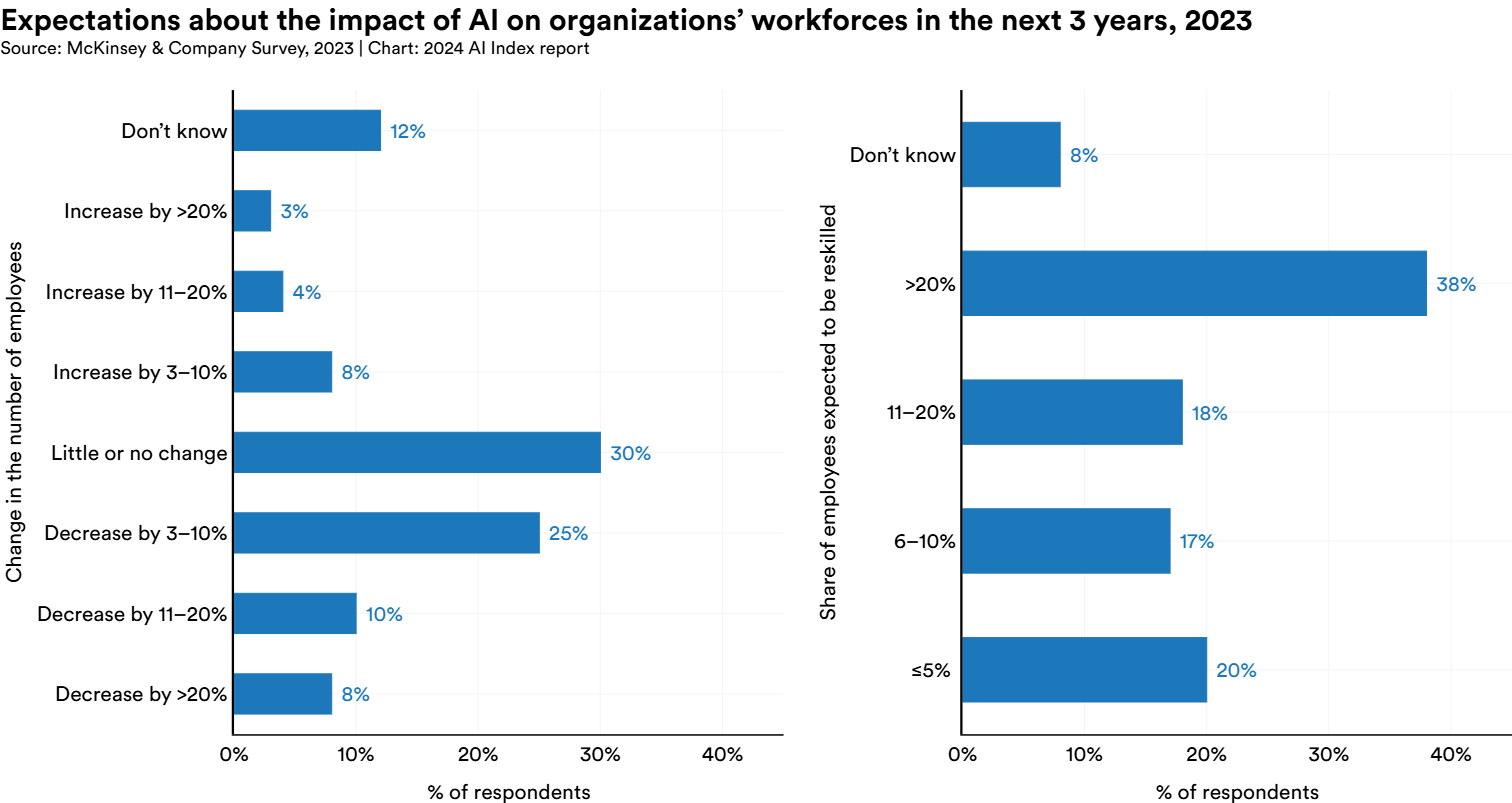
\includegraphics[width=0.7\linewidth]{figure/18未来3年人工智能对组织劳动力影响的预期图.png}
    \caption{未来3年人工智能对组织劳动力影响的预期图}
    \label{未来3年人工智能对组织劳动力影响的预期图}
\end{figure}

图表左侧展示了未来三年内,AI对员工数量变化的预期。其中有38\%的受访者认为,随着AI技术的推广,员工数量将增加超过20\%,这显示出许多企业对AI在提升劳动效率和创造就业机会方面充满信心;30\%的受访者则认为AI对员工数量的影响较小;而25\%的受访者预计,AI的应用可能使部分岗位受自动化或优化影响,导致员工数量下降3\%-10\%。

图表右侧则反映了关于AI对员工再培训需求的预期数据,38\%的受访者认为,超过20\%的员工需要接受再培训以适应技术变革,仅8\%的受访者对此持不确定态度。这表明,企业普遍认识到在AI日益普及的趋势下,员工技能升级成为必然选择。

总体而言,数据揭示了AI技术对劳动力市场的双重影响:一方面,它有望大幅提升生产力并带来更多高技能岗位;另一方面,低技能岗位可能面临被替代的风险。为此,各国企业和政府应提前制定措施,加强员工再培训和技能提升,以平衡技术进步带来的机遇和挑战。

\subsection{研发人员数量变化与科技创新推动的关系}
随着中国经济的持续增长和科技创新的不断推进,工业企业的研发投入和人才培养已成为衡量企业竞争力的重要标准、推动产业升级的关键。基于国家统计局以及和鲸平台的数据集《规模以上工业企业的科技活动基本情况》,制作出“2004-2023年中国规模以上工业企业研发人员数量的变化趋势”的柱状图(见图\ref{中国规模以上工业企业研发人员规模变化趋势图})。
\begin{figure}[H]
    \centering
    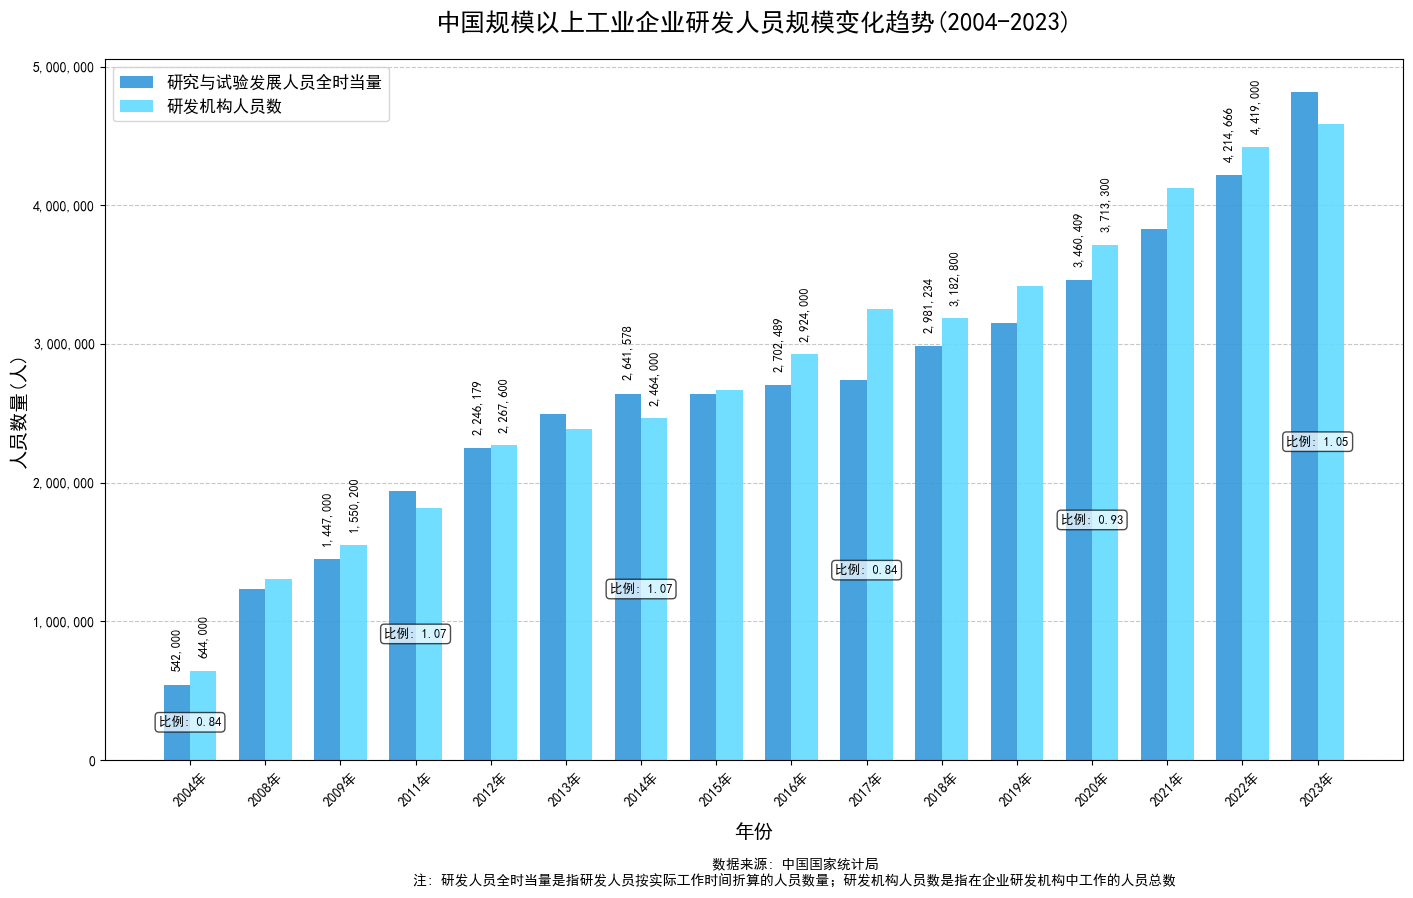
\includegraphics[width=0.6\linewidth]{figure/19中国规模以上工业企业研发人员规模变化趋势图.png}
    \caption{中国规模以上工业企业研发人员规模变化趋势图}
    \label{中国规模以上工业企业研发人员规模变化趋势图}
\end{figure}
从图表数据来看,2004年至2023年间,中国研发人员数量整体呈现稳定上升的趋势。尤其自2010年以后,研发人员数量的增长速度明显加快,2023年达到420万人以上,与2004年不足100万的水平相比增幅显著。这一增长趋势充分反映了中国对科技创新的高度重视,以及工业企业在技术研发方面的持续投入。

此外,近年来研发人员全时当量与机构人员数量均呈上升态势,甚至出现全时当量超过机构在岗人数的情况,显示出研发投入正逐步向灵活用工转变,并体现就业结构的多样化发展趋势。在年度对比中,研发人员占总员工数的比例逐步上升,尤其在2011年至2023年间,该比例不断接近甚至超过1.0,表明越来越多的企业将研发和创新作为提升竞争力的重要布局,特别是在高端制造业和高技术行业中,研发人才的重要性愈发凸显。\cite{li2023rd}

随着制造业智能化转型的不断推进和技术的持续发展,预计未来对研发人员的需求将持续增加。中国规模以上工业企业研发人员数量的稳步增长,不仅证明了国家在推动科技创新和产业升级方面取得的成效,也为企业转型升级、提高整体创新能力提供了坚实支撑。未来,研发人员数量的不断提升将成为推动中国经济高质量发展的重要驱动力。

\subsection{各产业就业人数变化}
在科技创新的强大驱动下,研发与人工智能岗位迅速增长,传统岗位正经历转型升级,为产业结构优化和经济高质量发展提供了强劲动能。基于国家统计局《按三次产业分就业人员数》数据集,制作出“2012-2023年中国各产业就业人员变化情况”的柱状图(见图\ref{各产业就业人员变化}),直观展示了这一时期内各产业就业人员的动态变化。
\begin{figure}[H]
    \centering
    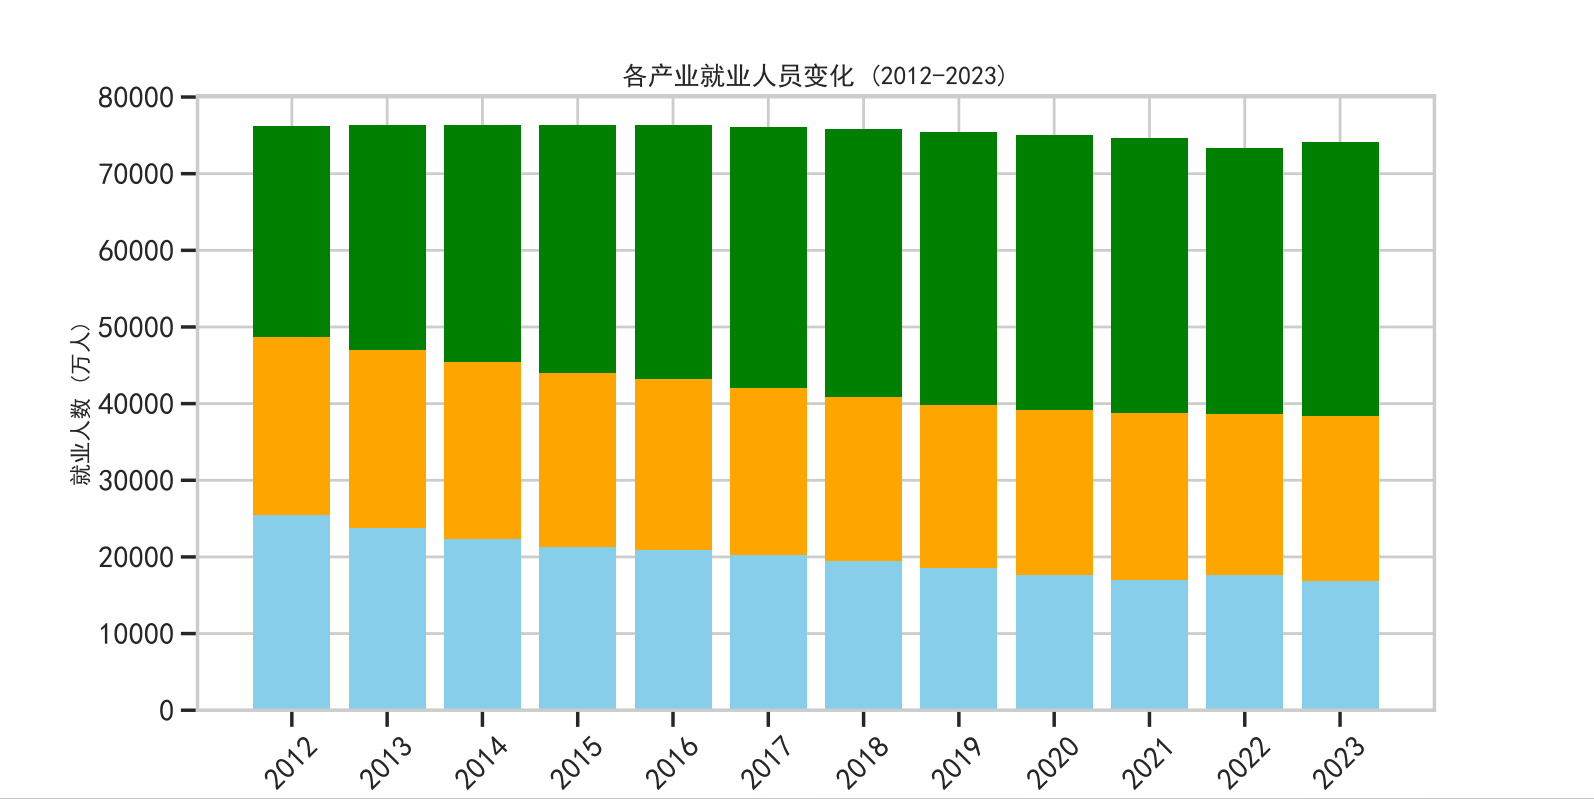
\includegraphics[width=0.7\linewidth]{figure/20各产业就业人员变化.png}
    \caption{各产业就业人员变化图}
    \label{各产业就业人员变化}
\end{figure}
从图中可以看出,随着中国经济的转型升级,劳动力市场正经历着由农业和制造业向服务业和高技术产业的结构调整。数据显示,第一产业就业人数持续下降,这与农业现代化、农村劳动力向城市转移密切相关;第二产业就业人数虽有波动,但总体呈下降趋势,反映出制造业中劳动力密集型岗位的逐步减少和产业结构的不断优化;而第三产业就业人数则稳步上升,尤其自2017年后服务业就业显著增长,预示着经济转向以高技术和服务导向为主的方向。

展望未来,随着数字经济和高技术行业的进一步发展,服务业与高端制造业将持续成为中国就业市场的主导力量。面对这种趋势,政府亟需加强对劳动力转型的支持,提升技能培训质量,促进人力资源在新兴行业中的高效配置,从而为经济高质量发展提供有力保障。